\chapter{Extend's Internal Architecture}

\begin{center}
  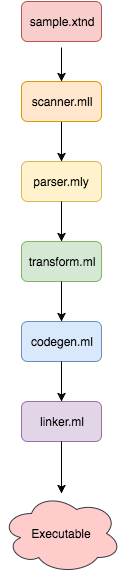
\includegraphics[width=.20\textwidth, height=15cm]{img/Execution.png}
\end{center}

\newpage

\section{The Extend Compiler}
The Extend compilation process consists of several source files, each of which performs a different function in the compilation pipeline.

\begin{itemize}
  \item \texttt{scanner.mll}: OCamllex scanner - consumes tokens.
  \item \texttt{parser.mly}: OCamlyacc parser - represents the Extend grammar.
  \item \texttt{ast.ml}: Abstract Syntax Tree, created from the output of the parser and representing the structure of an Extend program.
  \item \texttt{transform.ml}: Performs syntactic desugaring for easier compilation.
  \item \texttt{semant.ml}: Analyzes the semantics of the program to ensure that the program adheres to the rules of the language.
  \item \texttt{codegen.ml}: The LLVM IR code generator.
  \item \texttt{linker.ml}: Calls intermediary compilation steps on the generated \texttt{.ll}, including external functions if needed.
\end{itemize}

  \subsection{The Scanner}
  The function of \texttt{scanner.mll} is to parse a text stream into various tokens to be used in an Extend program.
  Only the tokens that are valid in Extend are to be given to the parser; all others will return a syntax error marked by the line and character number.

  \subsection{The Parser and Abstract Syntax Tree}
  The parser converts the tokens read by the scanner into a syntax tree deemed acceptable grammar within the Extend Language. This is converted into an Abstract Syntax Tree, which has nodes that can be consumed by the back end of the Extend compiler.

  \subsection{The Transformer}
The transformer is the first step in converting the AST into LLVM code. It takes the AST and reduces its breadth. This step is done to preserve the convenience for the user, but reduces the complexity for the actual compile step. It's important to note that the amount of transformation here is large; every expression on the left hand side, even if just a single number, gets turned into a variable.

  \medskip \noindent This is how the user declares a variable.
  \begin{lstlisting}
    [2,2] foo;
  \end{lstlisting}

  \medskip \noindent This is how the transformer desugars the same code.
  \begin{lstlisting}
    rows_of_foo := 2;
    cols_of_foo := 2;
    [rows_of_foo, cols_of_foo] foo;
  \end{lstlisting}

  \medskip \noindent
  Every expression before or after a comma or colon will become an internal temporary variable in the desugaring process. The transformer also transforms \texttt{\&\&, ||, and switch} into ternary conditionals to enable short-circuiting. Lastly, the transformer performs some semantic analysis to ensure that there are no duplicate variables within a function, and no duplicate functions within a program.

  \subsection{The Semantic Analyzer}
  The semantic analyzer consumes the reduced AST. It ensures that Extend functions, variables, expressions, and more are being used properly at compile time, and throws flavorful exceptions to the user so that they may better understand why their program was illegal. In Extend, there are no real type errors, as we attempt to degrade many gracefully. However, the semantic analyzer ensures that functions exist and have the right number of arguments, and that identifiers refer to real variables within their scope.

  \subsection{The Code Generator}
 Once the Extend AST passes semantic analysis, the code generator turns the reduced AST into LLVM code. Since the variable evaluation approach of Extend is not imperative, this process is fairly elaborate. Specifically for each Extend function it creates a collection of variable blueprints. In its most basic form each blueprint has a reference to one or more formulas that calculate the value of the variable. The intrinsics of this approach are beyond the scope of this overview.

  \subsection{The Linker}
  If successful LLVM IR is generated, the linker will adopt the role of building an executable object from the \texttt{.ll} file. This includes compiling it to an object file and linking the runtime environment along with other imported libraries.

  \section{Extend Runtime}
  % Should talk about runtime.c here
  Once a function is called, it recursively looks up what the return value depends on and calculates those values. For this process it is vital that the blueprints created by the Code Generator are correct. The algorithm uses those blueprints to instantiate relevant variables. Ultimately this allows very efficient calculation of the return value without understanding the underlying system.

  \medskip \noindent
  Take three arguments - scope, row, and cell. This lets the function refer to other local variables in that function. The function \texttt{getVal} tells us whether we can actually run the function or not.

  \medskip \noindent
  We generate code for every single variable in every single function.
